% State of the art, nåværende teknologi og implementasjoner
\section{Current state of XQuery}
\underline{\textbf{\LARGE //TODO:}} fylles ut, omstruktureres

There exist a number of XQuery implementations, few however are extended with full text capabilities. This section will briefly present some of the more prominent alternatives.
\subsection{Implementations with full-text extensions}
\subsubsection{Quark / TexQuery}
\begin{figure}[!h]
  \centering
    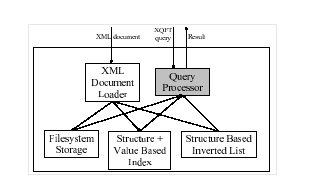
\includegraphics[width=0.5\textwidth]{img/quark_architecture.png}
  \caption{Quark architecture}
\end{figure}
Quark is an experimental full-text search engine capable of indexing and querying XML documents, and it uses the TexQuery query language (see below). Quark was developed as a research project at Cornell University by Jayavel Shanmugasundaram and his associates.
\begin{figure}[!h]
  \centering
    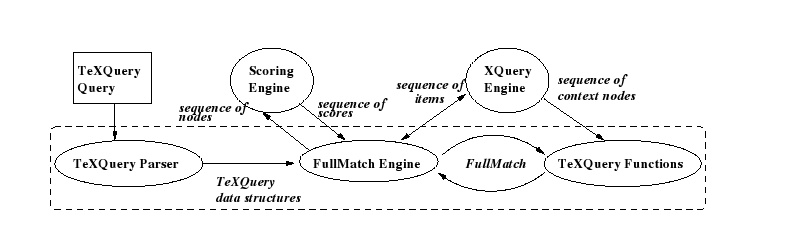
\includegraphics[width=1\textwidth]{img/texquery_architecture.png}
  \caption{TexQuery architecture}
\end{figure}
TexQuery is a query language extending upon Xquery with added full-text search capabilities. These extensions do not necessarily conform to the W3C recommendation, however TexQuery is an early precursor to the current W3C recommendation \cite{TEXQ00}, in whose development Shanmugasundaram actively participates.

\subsubsection{Galatex}
\begin{figure}[!h]
  \centering
    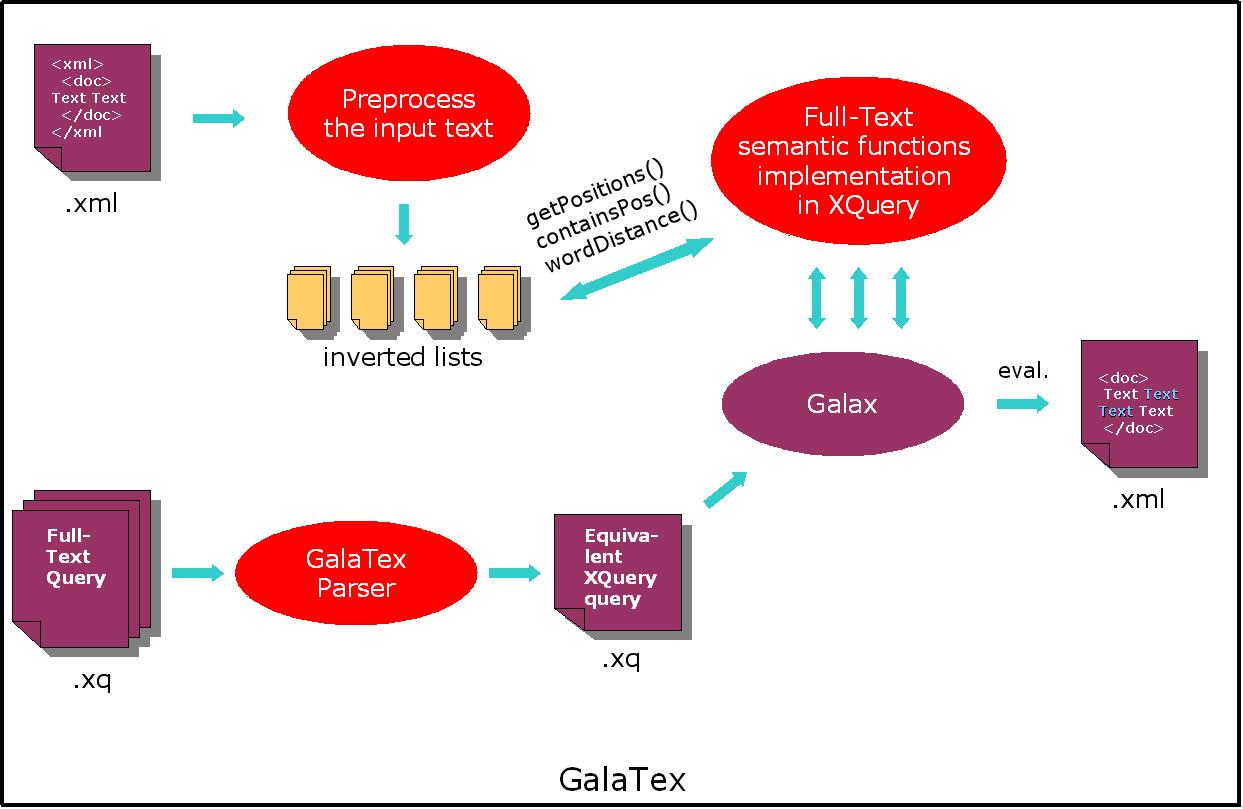
\includegraphics[width=1\textwidth]{img/galatex_architecture.png}
  \caption{Galatex architecture}
\end{figure}
GalaTex is a complete implementation of the Xquery 1.0 and Xpath 2.0
specifications with full-text extensions. GalaTex is an extension of Galax,
which is a generic Xquery engine. The XQFT query is parsed and converted to an
equivalent Xquery query which is passed to the Galax query engine. The GalaTex
source code is licensed under a non-commercial license developed to AT\&{}T 
\footnote{http://www.galaxquery.com/galatex/LICENSE} and is available at the
GalaTex website \cite{galatex}.

\subsubsection{Pathfinder}
\begin{figure}[!h]
  \centering
    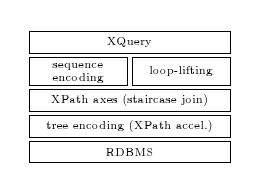
\includegraphics[width=0.5\textwidth]{img/pathfinder_architecture.png}
  \caption{Pathfinder architecture / development stack}
\end{figure}
The Pathfinder project is an XQuery parser running on top of relational database systems, namely MonetDB. The goal of the Pathfinder project is to investigate how relational database technology can be utilized to create a scalable and efficient XQuery implementation. However, the Pathfinder project has, at the current time of writing, no support for full text extensions. A future version of Pathfinder is planned to be capable of emitting SQL code generated from the XQuery parse tree. This illustrates the Pathfinder systems capabilities of interoperating with relational database systems.

Pathfinder is written in C, and the XQuery parser is a generated using standard Flex and Bison compiler generator tools.

\subsubsection{SaXon}
SaXon is an open source XSLT and XQuery processor. It is being actively developed by Michael Kay, and is licensed under the Mozilla Public License (MPL). SaXon conforms to the XSLT 2.0, XQuery 1.0 and XPath 2.0 recommendations by the W3C as of 23rd of january, 2007.

\subsubsection{Natix}
\begin{figure}[!h]
  \centering
    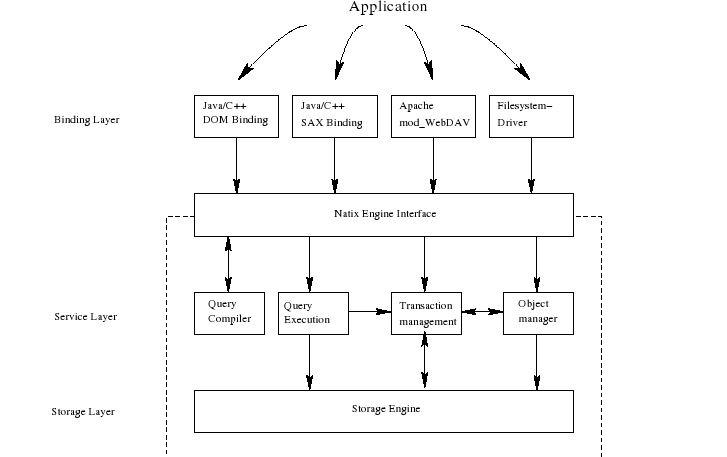
\includegraphics[width=1\textwidth]{img/natix_architecture.png}
  \caption{Natix architecture}
\end{figure}
Natix is an XML database system for persistent storage of XML, and provides access through DOM and SAX interfaces, as well as the option of performing XPath queries.